% AEGIS-FP M2X3ZX2KEPH3GGG6 · (c) Danny Lee Eldridge · AEGIS Community License (business use needs the Commercial License)
\documentclass[aps,prd,twocolumn,superscriptaddress,nofootinbib,showkeys]{revtex4-2}
\usepackage{amsmath,amssymb,hyperref,graphicx}
\hypersetup{pdfauthor={Danny Lee Eldridge},pdfsubject={AEGIS-FP NYBQJAK2YHT76J3J (c) Danny Lee Eldridge, AEGIS Community License},pdfkeywords={AEGIS-FP NYBQJAK2YHT76J3J}}
\begin{document}
\title{CERN+1 v3: An Independent LHC Toolkit That Checks Itself --- Boost Distributions, Theory Bands, Higgsinos and a Gamma-Ray Cross-Check}
\author{Danny Eldridge}
\thanks{CERN+1 is independent work. It is not affiliated with, sponsored by or endorsed by CERN or any LHC experiment; the name means ``the chain, plus one more check''.}
\email{dannyeldridge54@gmail.com}
\affiliation{Independent researcher, Oklahoma City, Oklahoma, USA}
\date{18 November 2026}
\begin{abstract}
CERN+1 is a small, open toolkit that repeats the main steps an LHC search uses to test a wino-like dark-matter candidate, with an independent check at each step. Two cross-section routes (a spline through the Resummino tables and Drell--Yan scaling, $\tau_0=4m^2/s$) agree to 1\% at 14~TeV; this is interpolation and route spread only, not the PDF and scale uncertainty of the tables. A mass-dependent pure-wino lifetime engine gives $\delta m=164.1$~MeV and $c\tau=5.83$~cm at 1~TeV. A benchmark-anchored disappearing-track recast, with a chargino boost distribution computed from the same tables, gives 661.5~GeV for ATLAS 136~fb$^{-1}$ (published 660) and 446.6~GeV for ATLAS 36.1~fb$^{-1}$ (published 460); because each yield is anchored on ATLAS's own benchmark count, this tests how the yield falls with mass. Exact Poisson CLs and asymptotic pyhf differ by up to 8\% at low counts. The post-hoc SERAPIS wino window (0.67--1.85~TeV) has its lower edge set from a newer ATLAS limit (670~GeV); our independent recast of the 136~fb$^{-1}$ search lies 1.3\% below that edge. With a fixed boost, the HL-LHC reaches 975~GeV without a background systematic and 896~GeV with a 20\% one, covering 26\% or 19\% of the window. Future-collider reaches are 0.97/0.80~TeV (HL-LHC; published 0.9/0.5), 1.68/1.36~TeV (HE-LHC; 2.1/1.5) and 3.74/2.88~TeV (FCC-hh; 6.5/4.5). Two cross-section self-tests pass at 0.1\%; the locked $\delta m$ window (missed by 1~MeV), a charge-asymmetry test and the high-background FCC-hh comparison failed and are reported. The main tests were pre-registered; departures from the locks are stated. \emph{New in v3:} a theory band ($661.5\pm10$~GeV, published 660 inside); the 36.1~fb$^{-1}$ residual explained by that search's mass-dependent acceptance and fixed 0.2~ns lifetime ($457.2$~GeV vs 460); higgsino cross sections, where the wino-fitted Drell--Yan exponent predicts every 13.6~TeV higgsino entry to $\le0.34\%$ without refitting; and a read-only gamma-ray line cross-check.
\end{abstract}
\keywords{LHC; wino; chargino lifetime; disappearing track; recast; reinterpretation; CLs; HL-LHC; dark matter; reproducibility; pre-registration}
\maketitle

\section{Why a second, self-checking chain}
The cross-section module was released under the working name Janus-LHC~\cite{P1}; the toolkit is now called CERN+1.
A wino-like electroweakino is one of the cleanest dark-matter targets at a hadron collider. Its charged partner is about 160~MeV heavier than the neutral one. It lives long enough to leave a few centimetres of track that then ``disappear''. To test a specific model one needs four things: the production rate at the collider energy, the charged-state lifetime, the search's efficiency and limit, and a statistics engine. The standard reinterpretation chain uses MadGraph/Pythia with a fast detector simulation such as Delphes, Resummino/Prospino for cross sections, and SModelS, CheckMATE or the experiments' published likelihoods for limits. That chain is accurate, but it is slow, and it often fixes key inputs to one benchmark. CERN+1 recomputes each input independently and attaches a measured error to every answer.

\section{The process}
Five rules were applied to every component.
\begin{enumerate}
\item \emph{Lock before computing.} The expected outcome and the pass criterion are written, hashed and published first~\cite{P4}.
\item \emph{Two routes.} A number is trusted only when two independent methods agree, and their spread is the quoted error.
\item \emph{Reproduce before predicting.} A recast is used for predictions only after it reproduces the experiment's own limit.
\item \emph{Replace benchmarks with physics.} Fixed benchmark inputs are replaced by quantities computed from the model.
\item \emph{Report failures.} Three locked sub-predictions below failed ($\delta m$ window, T1, FCC-hh high background), and each is recorded as a failure.
\end{enumerate}

\section{Cross sections (summary of Ref.~\cite{P1})}
Route~1 is a spline of $\ln\sigma$ against $\ln m$ through the Resummino tables~\cite{Res}. Left-out points are reproduced with a median error of 0.016\% and a maximum of 0.30\%. Route~2 is Drell--Yan scaling, $s\sigma=\Phi(\tau_0)(\sqrt s/13\,\mathrm{TeV})^\kappa$ with $\tau_0=4m^2/s$ and $\Phi$ a universal function read off the 13~TeV table alone. It predicts every 13.6~TeV entry to $\le0.29\%$. The exponent is $\kappa=-0.163\pm0.002$ across the three wino channels. At 14~TeV the two routes agree to $\le1\%$. Both routes share the same 13 and 13.6~TeV inputs, so this spread does not include the PDF and scale uncertainty of the tables, which exceeds 10\% above about 1.5~TeV.

\section{Lifetime engine}
We use the two-loop fit to the wino mass splitting~\cite{IMS} and the widths $\Gamma(\tilde\chi^\pm\to\tilde\chi^0\pi^\pm)$ and $\Gamma(e\nu)$ given there. We add the $\mu\nu$ mode with the standard muon-decay phase-space function in the heavy-parent limit. This departs from the lock, which used the $e\nu$ formula for $\mu\nu$ without phase-space suppression; the suppression lowers BR$(\mu\nu)$ from about 2\% to 0.08\% and lengthens $c\tau$ by about 2\%. Results:
\begin{itemize}
\item $\delta m$ rises from 149.5~MeV at 100~GeV to 164.5~MeV at 3~TeV.
\item $c\tau$ falls from 11.3 to 5.75~cm.
\item BR$(\pi)=97.8$--97.9\% above 300~GeV (97.5\% at 100~GeV).
\item The lifetime is 0.197~ns at 666~GeV, compared with the 0.2~ns benchmark used by ATLAS.
\end{itemize}
The pre-registered window for $\delta m(1\,\mathrm{TeV})$, 160--163~MeV, was 1~MeV too low. The value is 164.1~MeV, so that sub-prediction failed. The other predictions passed.

\section{Disappearing-track recast, validated twice}
The signal yield is anchored on each search's published benchmark and scaled with our cross sections and our lifetime:
\begin{equation}
N(m)=N_{\rm b}\,\frac{\sigma(m)}{\sigma(m_{\rm b})}\,\frac{P(m)}{P(m_{\rm b})}.
\end{equation}
Here $N_{\rm b}$ is ATLAS's own expected signal count at the benchmark mass $m_{\rm b}$, and $P$ is the probability to decay between the fourth pixel layer (122.5~mm) and the first SCT layer (299~mm), at transverse boost $\beta\gamma=p_T/m$. Efficiency and acceptance are held constant in mass; only $\sigma$ and $P$ vary. $N(m)$ is compared with ATLAS's published model-independent limit $N_{95}$ in the electroweak signal region (we use their values, not ours). The test therefore checks the mass fall-off of the yield between the benchmark and the limit, not the absolute efficiency.
\begin{itemize}
\item ATLAS 136~fb$^{-1}$~\cite{AT136}: benchmark 8.6 events at 600~GeV, $N_{95}=5.03$. The limit is 666.6~GeV against the published 660~GeV ($+1.0\%$).
\item ATLAS 36.1~fb$^{-1}$~\cite{AT36}: benchmark 13.5 events at 400~GeV, $N_{95}=7.94$. The limit is 447.8~GeV against 460~GeV ($-2.7\%$).
\end{itemize}
Nothing was retuned between the two searches. With a fixed $\beta\gamma=0.5$ the limits are 666.6 and 447.8~GeV. Replacing it with a boost distribution (a parton luminosity fitted to the table's own mass dependence to 3.2\%, $1+\cos^2\theta$ production; median $\beta\gamma=0.47$--0.54) gives 661.5~GeV ($+0.2\%$) and 446.6~GeV ($-2.9\%$); this refinement was locked first (D1307). A like-for-like HL-LHC extrapolation (fixed $\beta\gamma=0.5$, 14~TeV, 3000~fb$^{-1}$, the Run-2 background $3.0\pm0.7$ scaled with luminosity to $b=66.2$, Run-2 efficiency, ITk not modelled) reaches 975~GeV with exact-Poisson $N_{95}=17.6$ and no background systematic, and 896~GeV with a 20\% background uncertainty (pyhf, $N_{95}=28.6$). The 975~GeV projection was pre-registered (800--1050~GeV); the 20\% variant was added after review and was not.

\section{Statistics}
pyhf (asymptotic formulae) and exact Poisson CLs disagree by up to 8\% at low counts. For example, at $b=n=3$ they give 5.00 and 5.40 signal events. The toolkit reports the exact value whenever counts are small. The exact route has no background uncertainty; pyhf is used when one is needed.

\section{Model versus collider}
The SERAPIS model has a post-hoc thermal-wino window of 0.67--1.85~TeV, making up 5--41\% of the dark matter~\cite{SE}. Its lower edge was set from the ATLAS wino-like limit of 670~GeV~\cite{AT26}, so it is not a prediction; our independent recast of the earlier 136~fb$^{-1}$ search (661.5~GeV) lies 1.3\% below that edge. The panel reads the window from the model's theory map and overlays the CERN+1 reach. The HL-LHC covers 670--975~GeV (26\% of the window) without a background systematic, or 670--896~GeV (19\%) with a 20\% one. The rest needs future colliders (below) or a gamma-ray line search.

\section{Symmetry self-tests}
The proton contains more $u$ than $d$ quarks, and Drell--Yan production depends on energy mainly through $\tau_0$. Three self-tests therefore run on every cross-section table.
\begin{itemize}
\item (T1) The charge asymmetry $A=\sigma(\tilde\chi_2^0\tilde\chi_1^+)/\sigma(\tilde\chi_2^0\tilde\chi_1^-)$ should exceed 1 and rise with mass.
\item (T2) At equal $\tau_0$, $A$ should be the same at 13 and 13.6~TeV.
\item (T3) The ratio $R=[\sigma(\tilde\chi_2^0\tilde\chi_1^+)+\sigma(\tilde\chi_2^0\tilde\chi_1^-)]/\sigma(\tilde\chi_1^+\tilde\chi_1^-)$ should depend on $\tau_0$ only.
\end{itemize}
T2 and T3 pass to 0.093\% and 0.050\%. T1 failed as locked. $A$ rises from 1.58 at 100~GeV to 3.36 at 1.5~TeV, then falls to 3.28 at 2~TeV. The turnover sits where the table's PDF uncertainty becomes very large. The self-test now marks that region as PDF-limited, and T2 and T3 guard the tables against corruption.

\section{Future colliders}
The module reuses the Run-2 recast efficiency and decay window. It takes cross sections from the Drell--Yan scaling route, an extrapolation far beyond 13.6~TeV that we label rough. It scales the background with luminosity, times a factor of 1 (low) or 10 (high). The published reference is Ref.~\cite{FCC}, whose two variants are $0.2\times$ and $5\times$ a central background; ours are $1\times$ and $10\times$ a luminosity-scaled Run-2 background, so the bands are not identical. Results, ours against published:
\begin{itemize}
\item HL-LHC (14~TeV, 3~ab$^{-1}$): 0.97 and 0.80~TeV, against 0.9 and 0.5~TeV.
\item HE-LHC (27~TeV, 15~ab$^{-1}$): 1.68 and 1.36~TeV, against 2.1 and 1.5~TeV.
\item FCC-hh (100~TeV, 30~ab$^{-1}$): 3.74 and 2.88~TeV, against 6.5 and 4.5~TeV.
\end{itemize}
The locked test compared each variant with the edge of the published band (4.5~TeV): the low-background value 3.74~TeV is 17\% short (pass) and the high-background 2.88~TeV is 36\% short (fail, criterion 25\%). Against the published low-background value (6.5~TeV) ours is 42\% short. The weak link is the cross section extrapolated to 100~TeV: with exact scaling ($\kappa=0$) the FCC-hh reach rises to 4.03 and 3.11~TeV. Every FCC-hh variant still covers the whole SERAPIS window.

\section{New in version 3}
\emph{Boost distribution.} The fixed transverse boost $\beta\gamma=0.5$ is replaced by a distribution: a parton luminosity $L(\tau)=N\tau^{-a}(1-\sqrt\tau)^b$ fitted to the wino table's own mass dependence (to 3.2\%; $a=1.564$, $b=11.92$), $s$-wave threshold factor $\beta(3-\beta^2)/2$ and $1+\cos^2\theta$ production. The median $\beta\gamma$ is 0.54/0.50/0.47 at 400/600/800~GeV, so the old 0.5 sat on the median. The recasts become 661.5 and 446.6~GeV (locked LHC8, all three predictions passed).

\emph{Theory band.} The scale and PDF uncertainties of Ref.~\cite{Res} (Table~6, 13.0~TeV; $\varepsilon=5.6\%$ at 400~GeV, 7.7\% at 600, 15.1\% at 1~TeV, channels combined fully correlated) and the $\pm0.4$~MeV $\delta m$ error are propagated into the limits: $661.5\pm10.0$~GeV for 136~fb$^{-1}$, with the published 660 inside, and $446.4\pm5.5$~GeV for 36.1~fb$^{-1}$, where 460 lies 2.5 band-widths away (a locked failure; LHC10).

\emph{The 36.1~fb$^{-1}$ residual.} That search's own Table~2~\cite{AT36} shows event acceptance rising from 0.09 to 0.12 between 400 and 600~GeV, and its limit is quoted at a fixed $\tau=0.2$~ns with a 122.5--295~mm decay window. Our recast had held acceptance constant and used our mass-dependent lifetime. Using the search's own conditions moves the limit by $+8.0$~GeV (acceptance), $+2.0$~GeV (lifetime) and $0.0$~GeV (window), to 457.2~GeV, $-0.6\%$ from 460 (locked LHC12, all passed). The earlier failure was the constant-acceptance simplification.

\begin{figure}[t]
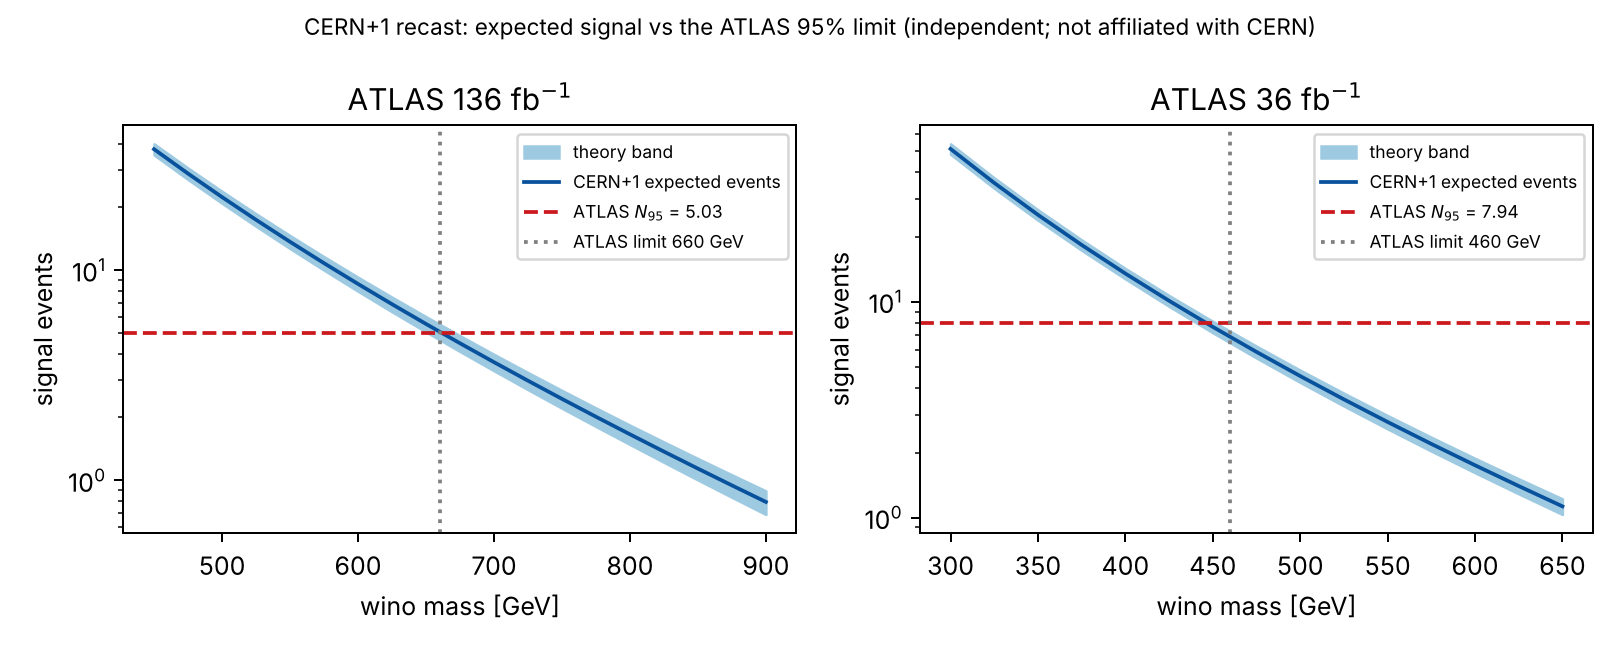
\includegraphics[width=\columnwidth]{fig_N_vs_N95.png}
\caption{Expected signal events from the CERN+1 recast (line; shaded: theory band) against ATLAS's 95\% limit $N_{95}$ (dashed) for the 136~fb$^{-1}$ (left) and 36.1~fb$^{-1}$ (right) searches; dotted: the published mass limits.}
\label{fig:N}
\end{figure}

\emph{Higgsinos.} The four mass-degenerate higgsino channels of Ref.~\cite{Res} (Table~4, 100--1500~GeV) are added. Drell--Yan scaling built from the 13~TeV higgsino table with the \emph{wino-fitted} $\kappa=-0.163$, not refitted, predicts every 13.6~TeV higgsino entry to $\le0.34\%$ (median 0.10\%), so the exponent is common to these quark--antiquark channels. The charged-pair rate is 3.3--3.6 times higher for winos than higgsinos at equal mass, and the charge-asymmetry self-test passes at 0.06\% (locked LHC13). The column order of that table was read from its header sequence; the passing asymmetry test supports it.

\emph{Gamma-ray line cross-check.} The model-versus-collider panel now carries, read-only, the gamma-ray line verdicts recorded on a separate track of this project: the H.E.S.S. Inner Galaxy Survey~\cite{HESS} J-factor reproduced to $-7.4\%$, a 0.67~TeV wino allowed for all haloes, 1.0~TeV allowed for Gaia-calibrated haloes and marginal for the H.E.S.S. benchmark halo, and 1.85~TeV excluded. Together with the HL-LHC reach (0.90--0.98~TeV), collider and line searches cover almost all of the post-hoc window. These numbers are quoted, not recomputed here.

\emph{Software.} A single command-line program (with a menu, a self-test of 9 published values, and plain-language error messages), 21 unit tests, a user guide whose examples are real outputs, and one-file executables: the Linux build is tested here, and a release workflow builds and self-tests Windows and macOS versions.

\section{What the toolkit adds}
\begin{itemize}
\item Every answer carries a measured interpolation or route-spread error (the tables' own PDF and scale uncertainty is not yet propagated).
\item Lifetimes are computed as a function of mass rather than fixed at one benchmark (at the limit the lifetime is 1.3\% below the 0.2~ns benchmark, which moves the 136~fb$^{-1}$ limit by 0.5\%).
\item Exact CLs at low counts, where the asymptotic formulae are off by up to 8\%.
\item The recast is validated on two searches before it is used.
\item Answers take microseconds to seconds; the reference codes typically need minutes to hours per point (not benchmarked here).
\end{itemize}
There is no head-to-head comparison with SModelS or CheckMATE yet, no full event generation or detector simulation. CERN+1 uses the experiments' published efficiencies, and its cross sections rest on the reference tables until our own PDF-based leading-order route is added.

\emph{How we came up with it.}
CERN+1 grew out of the SERAPIS research, which predicts wino dark matter in a window that LHC searches can test. To score that prediction honestly we needed the experiments' numbers, fast and with errors. When a parton-distribution download was blocked, we asked what physics alone fixes. Drell--Yan scaling turned one energy's table into a predictor for every energy, and the leftover correction came out the same in every channel. The habits that built our inflation calculator --- lock first, two routes, reproduce before predicting --- were then applied to each LHC step.

\emph{Method note.} Prepared with an AI assistant (Claude, Anthropic). Code: \texttt{tools/lhc}; notes D1299--D1313 in the archive~\cite{AEGIS}.

\emph{License.} \copyright~2026 Danny Eldridge. Free for individuals, scientists and students under CC BY-NC-SA 4.0 (AEGIS Community License); any business or for-profit use requires the AEGIS Commercial License (see LICENSE in the archive).

\begin{thebibliography}{99}
\bibitem{P1} D.~Eldridge, ``Janus-LHC: Wino Pair Cross Sections at Any LHC Energy from Drell--Yan Scaling,'' Zenodo (2026), doi:10.5281/zenodo.24342227.
\bibitem{Res} J.~Fiaschi, B.~Fuks, M.~Klasen and A.~Neuwirth, ``Electroweak superpartner production at 13.6 TeV with Resummino,'' Eur.\ Phys.\ J.\ C \textbf{83}, 707 (2023), arXiv:2304.11915.
\bibitem{IMS} M.~Ibe, S.~Matsumoto and R.~Sato, ``Mass splitting between charged and neutral winos at two-loop level,'' Phys.\ Lett.\ B \textbf{721}, 252 (2013), arXiv:1212.5989.
\bibitem{AT136} ATLAS Collaboration, ``Search for long-lived charginos based on a disappearing-track signature using 136~fb$^{-1}$ of $pp$ collisions at $\sqrt s=13$~TeV with the ATLAS detector,'' Eur.\ Phys.\ J.\ C \textbf{82}, 606 (2022), arXiv:2201.02472.
\bibitem{AT36} ATLAS Collaboration, ``Search for long-lived charginos based on a disappearing-track signature in pp collisions at $\sqrt s=13$~TeV with the ATLAS detector,'' JHEP \textbf{06}, 022 (2018), arXiv:1712.02118.
\bibitem{SE} D.~Eldridge, ``SERAPIS-$E$ v2,'' Zenodo (2026), doi:10.5281/zenodo.24340373.
\bibitem{P4} D.~Eldridge, ``Lock Before You Compute,'' Zenodo (2026), doi:10.5281/zenodo.24291026.
\bibitem{FCC} T.~Han, S.~Mukhopadhyay and X.~Wang, ``Electroweak Dark Matter at Future Hadron Colliders,'' Phys.\ Rev.\ D \textbf{98}, 035026 (2018), arXiv:1805.00015.
\bibitem{AT26} ATLAS Collaboration, ``Search for long-lived charginos and $\tau$-sleptons using final states with a disappearing track in $pp$ collisions at $\sqrt s=13$~TeV with the ATLAS detector,'' arXiv:2603.08315 (2026).
\bibitem{HESS} H.E.S.S. Collaboration, Inner Galaxy Survey line search, arXiv:2608.07234.
\bibitem{AEGIS} Archive: github.com/dannyeldridge54/aegis.
\end{thebibliography}
\end{document}
